\DiaryEntry{Scalar Quantization, 2}{2021-06-16}{Coding}

The basic idea of non-uniform quantization is to quantize signal intervals which have higher probability with more accuracy (closer quantizer intervals) and signals intervals which have lower probability with less accuracy (wider quantizer intervals). On average, the squared error will be reduced.

\subsection{PDF-optimized Quantization}

If we write down the quantization error $\sigma_q^2$,

\bee
\sigma_q^2 = \int_{- \infty}^\infty (x - Q(x))^2 f_X(x) dx = \sum_i \int_{b_{i-1}}^{b_i} (x - y_i)^2 f_X(x) dx
\eee

then we want to find those values of $b_i, i=0, \ldots M$ and $y_i, i=1, \ldots, M$ that minimize $\sigma_q^2$.

We can actually differentiate above expression wrt to $y_j$ and set it to zero and obtain

\bee
y_j = \frac{ \int_{b_{j-1}}^{b_j} x f_X(x) dx }{ \int_{b_{j-1}}^{b_j} f_X(x) dx }
\eee

The output point for each quantization interval is the centroid of the probability mass in that interval.

In a similar spirit, we can also differentiate wrt to $b_j$, set to zero, and obtain

\bee
b_j = \frac{y_{j+1} + y_j}{2}
\eee

The decision boundary is simply the midpoint of the two neighboring reconstruction levels. Solving these two equations will give us the values for the reconstruction levels and decision boundaries that minimize the mean squared quantization error. Unfortunately, to solve for $y_j$, we need the values of $b_j$ and $b_{j-1}$; and to solve for $b_j$, we need the values of $y_{j+1}$ and $y_j$.

The \emph{Lyod-Max} algorithm solves this problem in an iterative manner.

\subsection{Companded Quantization}

Instead of making the step size small, we could make the interval in which the input lies with high probability large—that is, expand the region in which the input lands with high probability in propor- tion to the probability with which the input lands in this region. This is the idea behind companded quantization.

The following Figure shows a block diagram.

\begin{figure}[H]
    \centering
    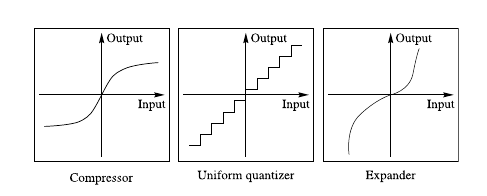
\includegraphics[scale=0.7]{images/2021-06-16-scalar_quant_01.png}
\end{figure}

For the following, we assume that input signal values near zero are more probable than larger input values.

The input is first mapped through a compressor function. This function “stretches” the high-probability regions close to the origin and correspondingly “compresses” the low-probability regions away from the origin. Thus, regions close to the origin in the input to the compressor occupy a greater fraction of the total region covered by the compressor. If the output of the compressor function is quantized using a uniform quantizer and the quantized value transformed via an expander function, the overall effect is the same as using a nonuniform quantizer.



%%% Local Variables:
%%% mode: latex
%%% TeX-master: "journal"
%%% End:
